\section{Durchführung}
\label{sec:Durchführung}

Der Versuchsaufbau ist in \autoref{fig:Messapparatur} schematisch dargestellt.
An der Vorrichtung befinden sich auf einer Schiene mit Längenskalierung zwei verschiebbare Messuhren, die die Auslenkung messen.
Zunächst werden die Massen und Maße der elastischen Stäbe mithilfe einer elektrischen Waage, eines Maßbandes und eines Messschiebers bestimmt.
Bei den Probekörpern handelt es sich um einen rechteckigen und einen runden Stab des gleichen Materials. 


\begin{figure}[H]
    \centering
    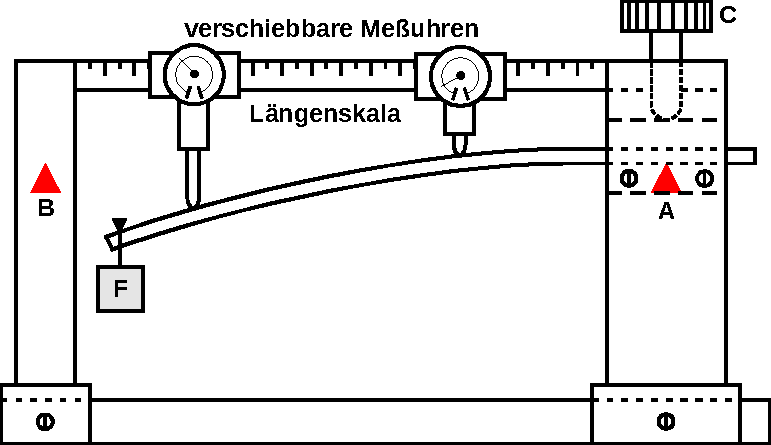
\includegraphics{content/Messapparat.pdf}
    \caption{Aufbau der Apparatur zur Messung der Durchbiegung der elastischen Stäbe.\cite[111]{V103}}
    \label{fig:Messapparatur}
\end{figure}

\subsection{Einseitige Einspannung}
Der Probekörper wird einseitig am Punkt C eingespannt. 
Am Ende des Stabes wird ein Gewicht angehangen, sodass sich der Stab durchbiegt. 
Hierbei soll eine maximale Auslenkung von $\num{3}$ bis $\qty{7}{\milli\meter}$ erreicht werden.
Es werden mehrere Messungen entlang des Stabes durchgeführt.
Da nicht davon ausgegangen werden kann, dass die Stäbe exakt gerade sind, werden die Messuhren vor jeder Messung der Auslenkung auf Null gesetzt,
bevor das Gewicht angehangen wird.
Nun wird die Auslenkung $D(x)$ bestimmt und in Abhängigkeit vom Abstand $x$ zur Einspannung in einer Tabelle notiert, 
bevor die Messuhren um einen Abstand von $\qty{2,5}{\centi\meter}$ verschoben werden.
$D(x)$ wird bestimmt durch die Formel
\begin{equation}
    D(x) = D_m(x) - D_0(x)
    \label{eqn:D(x)1}
\end{equation}
, wobei $D_0(x)$ hier Null ist, wenn die Messuhr vor jeder Messung auf Null gesetzt wird und $D(x)$ somit direkt abgelesen werden kann.

\subsection{Beidseitige Auflage}
Das Verfahren wird analog für die beidseitige Auflage wiederholt. Nun liegt der Probekörper jedoch auf den Punkten A und B auf und das Gewicht wird mittig 
angehangen anstatt am Ende des Stabes. Außerdem muss nun beachtet werden, dass an beiden Hälften des Stabes mit verschiedenen Messuhren gemessen wird.




